\section{Introduction}
In the beginning, there was FORTRAN.

\begin{figure*}
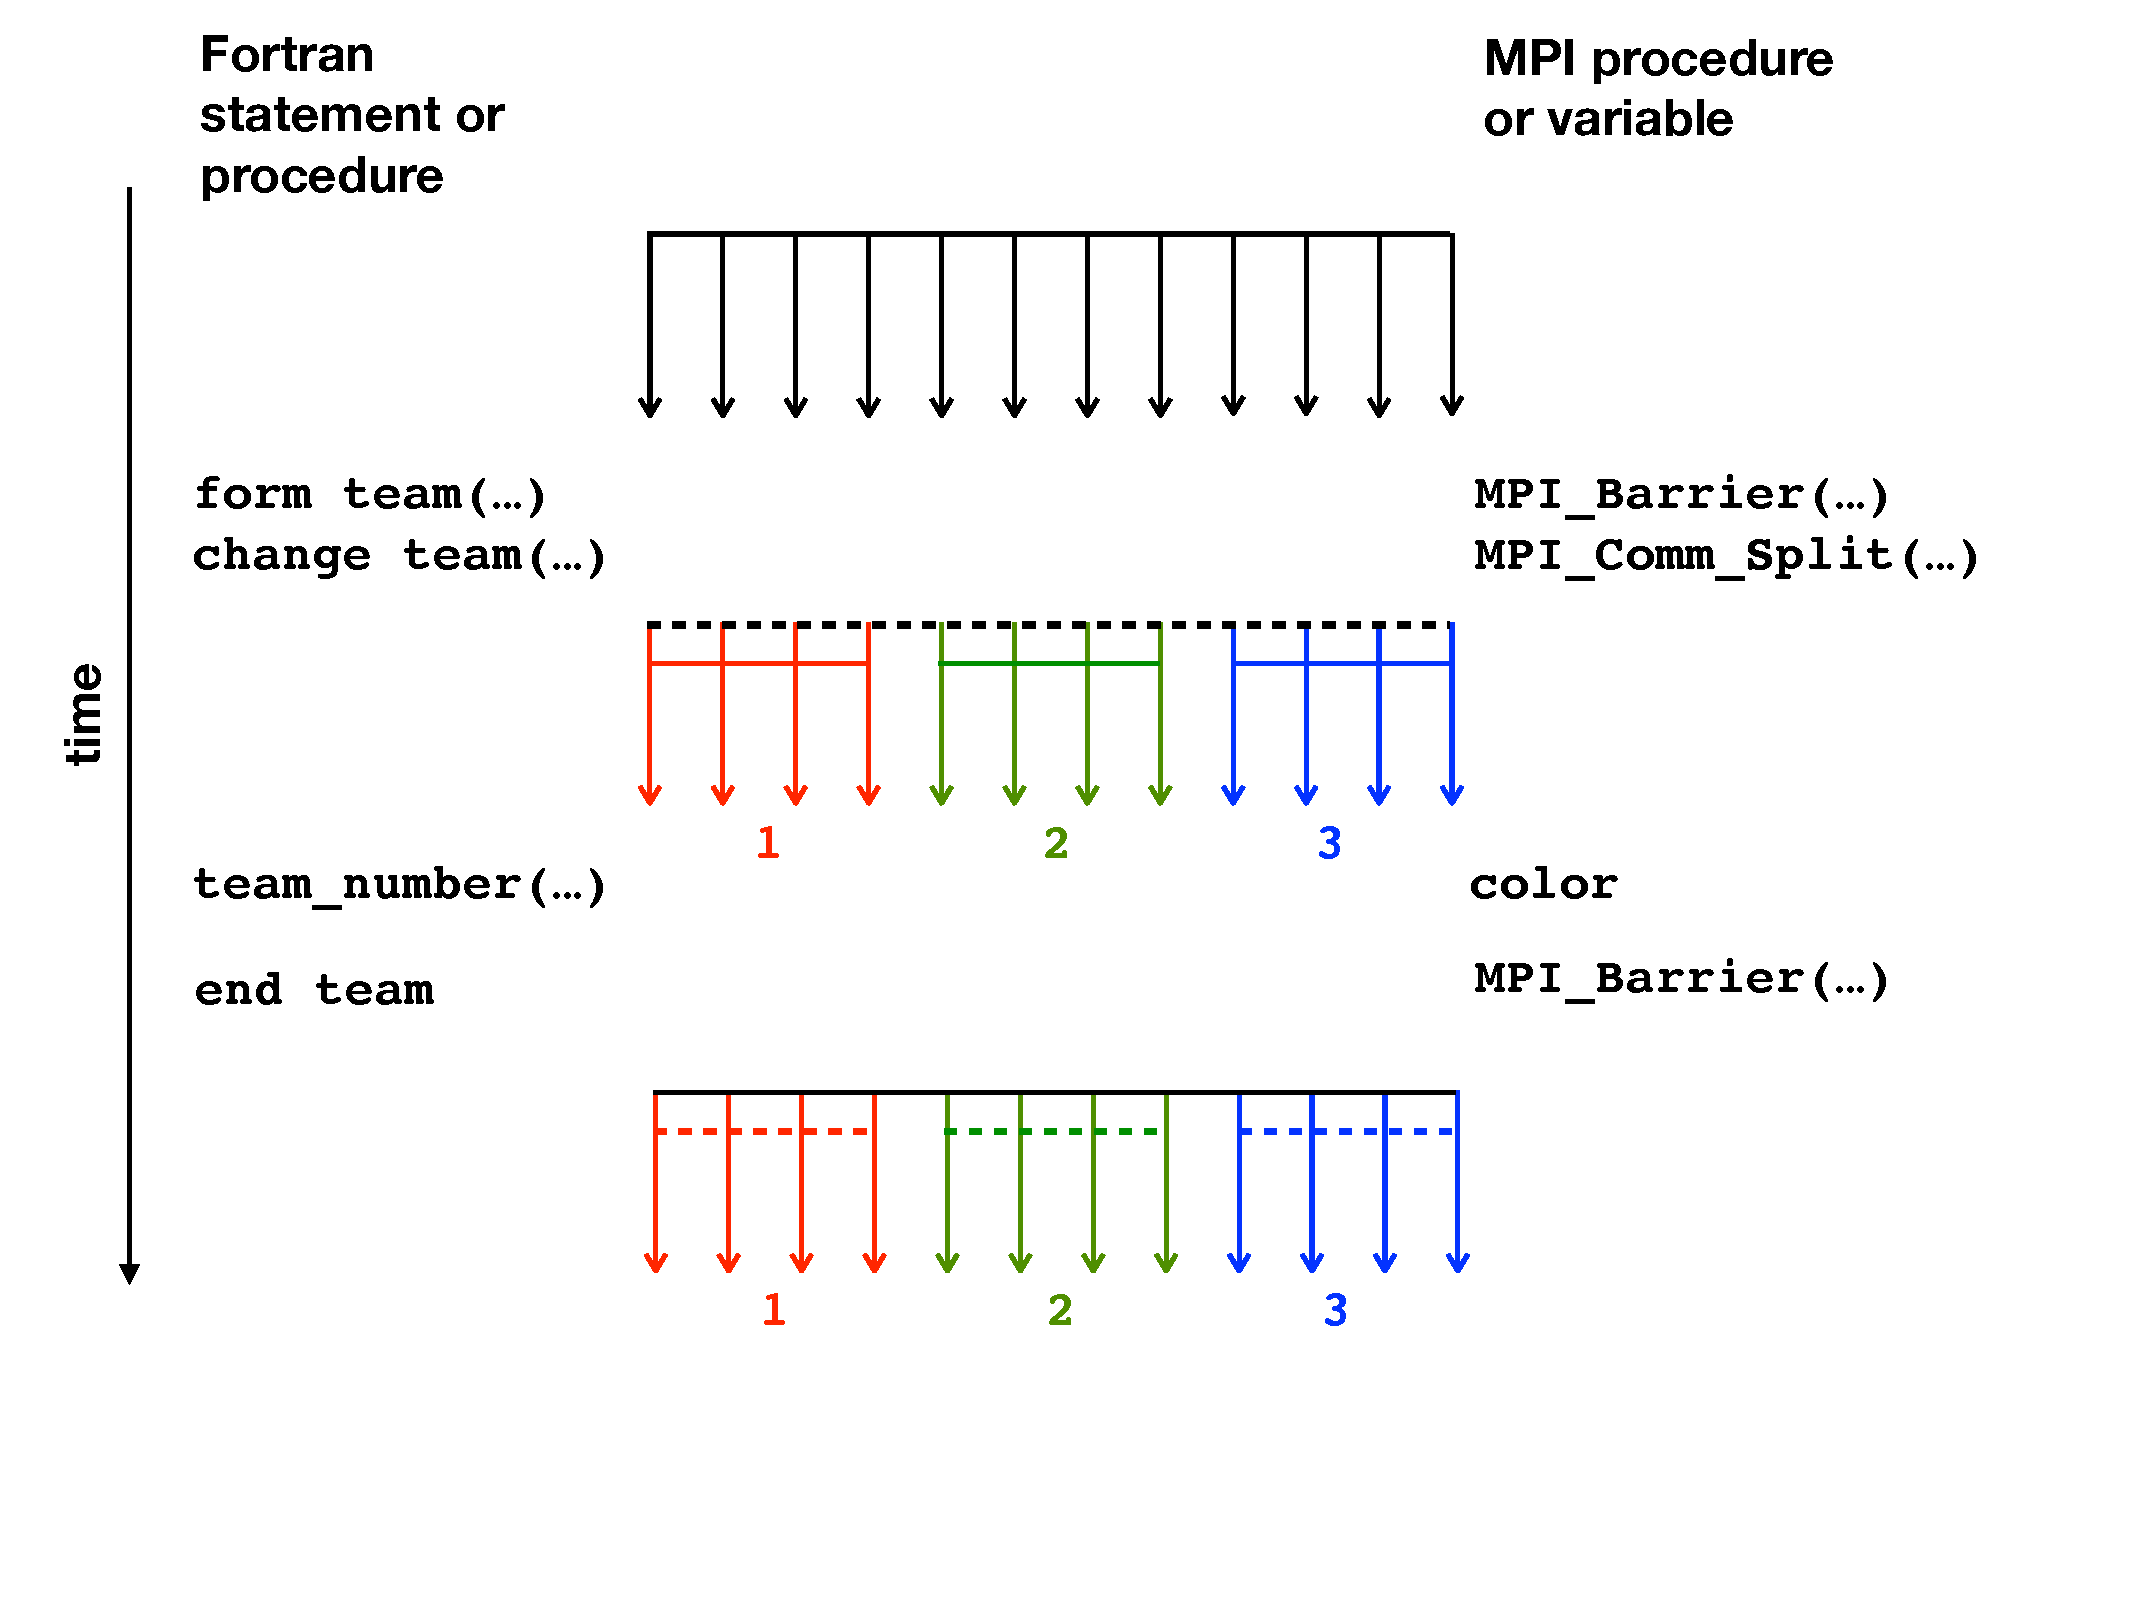
\includegraphics[width=0.7\textwidth]{figures/teams}
\vspace{-36pt}
\caption{Schematic depiction of a Fortran program executing over time (left axis) in 12 images (top) thatcommunicate with each other through global means (black horizontal bar) and later communicating within subgroups (colored horizontal bars).  Horizontal lines represent the communication mechanisms (default=solid, optional=dashed).  Fortran concepts or on the left.  The underlying \gls{mpi} concepts are the right.}
\end{figure*}
%

\begin{figure*}
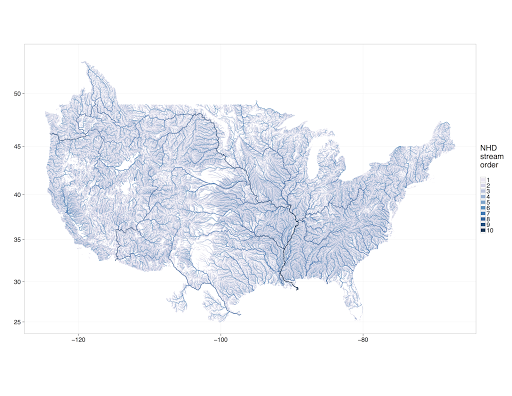
\includegraphics[width=0.7\textwidth]{figures/hydro-map}
\vspace{-36pt}
\caption{Sample WRF-Hydro simulation domain.}
\end{figure*}
%

%%%
%%% Sample tables
%%%

%\begin{table}
%  \caption{Frequency of Special Characters}
%  \label{tab:freq}
%  \begin{tabular}{ccl}
%    \toprule
%    Non-English or Math&Frequency&Comments\\
%    \midrule
%    \O & 1 in 1,000& For Swedish names\\
%    $\pi$ & 1 in 5& Common in math\\
%    \$ & 4 in 5 & Used in business\\
%    $\Psi^2_1$ & 1 in 40,000& Unexplained usage\\
%  \bottomrule
%\end{tabular}
%\end{table}

%\begin{table*}
%  \caption{Some Typical Commands}
%  \label{tab:commands}
%  \begin{tabular}{ccl}
%    \toprule
%    Command &A Number & Comments\\
%    \midrule
%    \texttt{{\char'134}author} & 100& Author \\
%    \texttt{{\char'134}table}& 300 & For tables\\
%    \texttt{{\char'134}table*}& 400& For wider tables\\
%    \bottomrule
%  \end{tabular}
%\end{table*}
% end the environment with {table*}, NOTE not {table}!

%It is strongly recommended to use the package booktabs~\cite{Fear05}
%and follow its main principles of typography with respect to tables:
%\begin{enumerate}
%\item Never, ever use vertical rules.
%\item Never use double rules.
%\end{enumerate}
%It is also a good idea not to overuse horizontal rules.


%%%
%%% Sample figures
%%%

%\begin{figure}
%\includegraphics{fly}
%\caption{A sample black and white graphic.}
%\end{figure}

%\begin{figure}
%\includegraphics[height=1in, width=1in]{fly}
%\caption{A sample black and white graphic
%that has been resized with the \texttt{includegraphics} command.}
%\end{figure}

%\begin{figure*}
%\includegraphics{flies}
%\caption{A sample black and white graphic
%that needs to span two columns of text.}
%\end{figure*}
%
%\begin{figure}
%\includegraphics[height=1in, width=1in]{rosette}
%\caption{A sample black and white graphic that has
%been resized with the \texttt{includegraphics} command.}
%\end{figure}

%\end{document}  % This is where a 'short' article might terminate



\appendix
%Appendix A
\section{Code listing}
% This next section command marks the start of
% Appendix B, and does not continue the present hierarchy
\section{Anything else?}

\begin{acks}
  The authors would like to thank the CISL and RAL Visitor Program

  The work is
  supported by the \grantsponsor{GSxxxxx}{National
  Science Foundation China}{http://dx.doi.org/zz.yyyyy/xxxxx} under Grant
  No.:~\grantnum{GSxxxxx}{yyyyyyy}

\end{acks}
